
%Here I need to go through and describe all of the things that are important for the discussion
%aim for 20 pages

%things to discuss include:
%- A general introduction to the standard model (probably no more than a page or two)
%- Electroweak physics
%- W decay
%- parton distribution functions (maybe with some thorough discussion on this) as well as renormalization and factorization scales

%- WWW production (do I actually want to discuss this at all here??)
%- Effective field theory and anomalous coupling measurements


%assuming these will be defined here
% Quartic Gauge Couplings (QGC) 
% Standard Model (SM)
% anomalous Quartic Gauge Couplings (aQGC)
% Parton Distribution Function (PDF)


\section{The Standard Model}

The Standard Model (SM) is a theory which describes all of the
observed matter and interactions in the universe, except for gravity.
It is built from a quantum field theory where the consitutent particles
and interactions fit into a non-Abelian 
$\suthree\times\sutwo\times\uone$~gauge symmetry.
From these symmetries come the matter fermions, split 
into the quarks and leptons, and the force-carrying bosons
that mediate their interactions.
The \suthree~symmetry describes the theory of Quantum Chromodynamics (QCD)
which explains the interaction of the quarks via the gluons, the
gauge bosons that mediate the strong force.
The remaining $\sutwo\times\uone$~symmetry 
describes the Electroweak (EW) theory which explains
the interactions of the quarks and leptons via the 
electroweak gauge bosons that mediate
the electroweak force: $W$, $Z$, and $\gamma$ (i.e. the photon).
The EW theory is itself a unified description of the weak force,
involving the $W$ and $Z$, and the electromagnetic force, involving
just the photon.
The $W$ and $Z$ gauge bosons (as well as the quarks and leptons) receive
their non-zero masses through the process of electroweak symmetry
breaking (EWSB). The simplest form of EWSB
introduces an additional 'Higgs' field that
predicts a single new fundamental scalar boson. This boson is the
famous Higgs boson which was discovered recently at the LHC, thereby
confirming this last component of the SM.
%cite

All of the 
observed fundamental 
matter particles in the universe are described by the quark
and leptons of the SM. Their properties are listed 
in \tab\ref{tab:theory_fermions}. 
The particles can be distinguished
by their charges and their masses.
The charges describe how (and if) the particles participate in
different interactions.
Those fermions with electric charge (all but the neutrinos) 
participate in the electromagnetic
interactions. The quarks have color charge (sometimes 
just called color), which allows them to 
participate in the QCD interactions. All fermions also participate in 
the weak interactions. The types of allowed weak interactions are determined
by a combination of the electric charge as well as the weak isospin
and weak hypercharge, described later.
%explain better
Since all of the particles are fermions, they all have a spin of 1/2.
The masses of the particles are not predicted by the theory, but 
are essential for understanding their stability and decay properties
as well as their kinematic behavior.
Each particle also has a corresponding anti-particle with the same mass but
whose electric charge has opposite sign. The neutrinos, with zero 
electric charge, could possibly be their own 
anti-particle (so-called Majorana fermions), but
this has yet to be confirmed.

\begin{table}[ht]
\centering
\small
\begin{tabular}{|lclc|c|c|}
\hline
                        & Generation & Name & Symbol  & Charge & Mass [MeV]\\
\hline
\hline
\multirow{6}{*}{Quarks}& \multirow{2}{*}{First}& Up & $u$   &  $~~2/3$    &  $2.3 ^{+0.7}_{-0.5}$    \\
                       & & Down & $d$  &  $-1/3$    &  $4.8^{+0.5}_{-0.3}$    \\
		       \cline{2-6} 
                       &\multirow{2}{*}{Second}& Charm & $c$   & $~~2/3$     & $1275 \pm 25$     \\
                       && Strange & $s$   & $-1/3$     & $95 \pm 5$     \\
		       \cline{2-6} 
                       &\multirow{2}{*}{Third}& Top & $t$   &  $~~2/3$    &  $173210 \pm 874$    \\
                       && Bottom & $b$   &  $-1/3$    & $4180 \pm 30$     \\
\hline
\hline
\multirow{6}{*}{Leptons}&\multirow{2}{*}{First} &Electron & $e$     &  -1    &  $0.510998928 \pm 0.000000011 $ \\
                        & & Electron Neutrino & $\nu_e$  & 0    &   $ < 0.002$    \\
		       \cline{2-6} 
                        &\multirow{2}{*}{Second} &Muon & $\mu$     &   -1   &   $105.6583715 \pm 0.0000035$   \\
                        & &Muon Neutrino & $\nu_{\mu}$  & 0   &  $ < 0.19$    \\
		       \cline{2-6} 
                        & \multirow{2}{*}{Third}&Tau & $\tau$     &   -1   &  $1776.86 \pm 0.12$    \\
                        & &Tau Neutrino & $\nu_{\tau}$  & 0    &  $< 18.2 $    \\
\hline
\end{tabular}
\label{tab:theory_fermions}
\caption{Summary of the electric charge and measured masses of the SM fermions. Mass measurements
are taken from the Particle Data Group \cite{PDG:2014} and 
are shown to the best precision available with their measured uncertainties.
Particles are also organized by their generation.
The bottom quark mass measurement is shown using the $\overline{\textrm{MS}}$ 
renormalization scheme.
The top quark mass uncertainty combines the reported statistical and systematic uncertainties 
in quadrature.
The limits on the electron neutrino and muon neutrino masses are set at a 90\% confidence level 
while the tau neturino limits are set at a 95\% confidence level.}
\end{table}

The quarks and leptons can each be divided up into three ``generations'' composed of pairs
of particles with identical charges but whose masses increase with each generation.
The generations are labeled in \tab\ref{tab:theory_fermions}. 
In the leptonic sector, leptons only interact exclusively with leptons of their own generation.
However, in the quark sector, while there is a strong preference for the quarks to interact
within the same generation, it is still possible for quarks to interact with quarks of 
the other generations. This is described by the CKM matrix... %elaborate
Even though there are three 
generations in both the lepton and quark sectors, 
the quarks and leptons are not observed to interact directly, 
thus the quark and lepton generations should be thought of as separate.


The SM can be written down using a lagrangian of the form
\begin{equation}
\curlyl_{\textrm{SM}} = \curlyl_{\textrm{QCD}} + \curlyl_{\textrm{EW}} + \curlyl_{\textrm{EWSB}}
\end{equation}
which is gauge invariant or something...
From this, one can calculate all of the fundamental interactions of the SM.
As written, the SM lagrangian can be split up into separate terms describing the
QCD, EW, and EWSB behavior. 
The EWSB term includes the behavior related to fermion mass generation.
The details of each term are described in more detail below.

CP violation?

\subsection{Quantum Chromodynamics}
The QCD term in the SM lagrangian can be written as
\subsection{Parton Distribution Functions}
\subsection{The Electroweak Theory}
\label{sec:theory_ew}
The electroweak (EW) theory of Glasgow, Weinberg, and Salam (cite)
is a renormalizable (cite t hooft?) 
is a non-Abelian gauge theory 
that successfully unifies the theories 
of \uone~electromagnetism and \sutwo~weak.
It incorporates the charge and parity violating interactions (cite?) 
of the weak interactions while preserving these symmetries of electromagnetism.
It explains the presence of the massive EW gauge bosons 
while maintaining gauge invariance
using spontaneous symmetry breaking via the Higgs 
mechanism which recently received confirmation through the discovery of 
the Higgs boson at the LHC in 2012 (cite). 
It also includes the CP violating flavor mixing of the 
charged interactions in the quark sector via the CKM (expand) matrix (cite).

   

V-A

The fermions of the electroweak field theory belong to doublets and singlets...
Describe R and L in advance

neutral current still has some 


The EW term in the SM lagrangian can be written as
\begin{equation}
\begin{aligned}
\curlyl_{\textrm{EW}} = &-\frac{1}{4}\textbf{W}_{\mu\nu} \cdot \textbf{W}^{\mu\nu} 
- \frac{1}{4} B_{\mu\nu} B^{\mu\nu}  \\
&+\overline{L}\gamma^{\mu}\Big( i \partial_{\mu} - g \frac{1}{2} \boldsymbol{\tau} \cdot \textbf{W}_{\mu} - g' \frac{Y}{2} B_{\mu} \Big) L \\
&+ \overline{R} \gamma^{\mu} \Big( i \partial_{\mu} - g' \frac{Y}{2} B_{\mu} \Big) R
\end{aligned}
\end{equation}
where the first two terms describe the kinetic energies and 
self-interactions of the EW gauge bosons
and the second two terms describe the fermion kinetic energies
and their interactions with the EW gauge bosons.
$L$ and $R$ (and their charge conjugates $\overline{L}$ and $\overline{R}$)
are the left-handed fermion isospin doublets and right-handed
fermion isospin singlets, described in more detail later.
The gauge fields, $\mathbf{W}_{\mu}$ and $B_{\mu}$, represent the 
massless EW gauge bosons before EWSB. They are four-vectors of the Lorentz group
and thus undergo Lorentz transformations as indicated by their Lorentz index $\mu$.
The $\mathbf{W}_{\mu}$ describes two charged gauge bosons and 
a neutral gauge boson as an isotriplet of 
vector fields ($W_{\mu}^i$)
in \sutwo~with generators
$\boldsymbol{\tau}$\footnote{The generators of \sutwo~are the famous
Pauli matrices.}.
The charged gauge bosons are represented by a superposition of the first
two componentns of the 
isotriplet, $W_{\mu}^{\pm}=\sqrt{\frac{1}{2}}\Big(W_{\mu}^1\mp i W_{\mu}^2\Big)$,
while the neutral gauge boson is represented 
by the third component, $W_{\mu}^3$.
The $B_{\mu}$ describes a single neutral gauge boson 
using a single vector field in \uone~with the generator $Y$, referred
to as the weak hypercharge.
By construction, the generator of \uone
electromagnetism, $Q$ (i.e. the electric charge), is related
to the generator of the third component of weak \sutwo, $T^3$,
and the weak hypercharge by $Q=T^3+Y/2$.
The $\partial_{\mu}$ is the four-dimensional partial derivative of the Lorentz
group and the $\gamma^{\mu}$ are the Dirac matrices.
The kinetic energies are described by the field strength tensors
\begin{equation}
\label{eq:wfieldstrength}
\textbf{W}_{\mu\nu} = \partial_{\mu}\textbf{W}_{\nu} - \partial_{\nu}\textbf{W}_{\mu} - g \textbf{W}_{\mu}\times \textbf{W}_{\nu}
\end{equation}
and 
\begin{equation}
B_{\mu\nu} = \partial_{\mu} B_{\nu} - \partial_{\nu} B_{\mu}
\end{equation}

The coupling constants $g$ and $g'$ describe the strength of the interactions
of the fermions with the gauge boson fields before EWSB. 

Upon EWSB, described in more detail in \sec\ref{},
the two neutral gauge boson fields, $W_{\mu}^3$ and $B_{\mu}$, 
mix according to the weak mixing angle, $\theta_W$:
\begin{align}
A_{\mu} =& \cos\theta_W B_{\mu} + \sin\theta_W W_{\mu}^3 \\
Z_{\mu} =& -\sin\theta_W B_{\mu} + \cos\theta_W W_{\mu}^3
\end{align}
where $Z_{\mu}$ corresponds to the massive $Z$ boson field
and $A_{\mu}$ corresponds to the massless photon field.
The charged $W$ bosons also receive a mass.
The masses of the $W$ and $Z$ and related by the weak mixing angle:
\begin{equation}
\frac{M_W}{M_Z} = \cos \theta_W
\end{equation}
as are the coupling constants, $g$ and $g'$:
\begin{equation}
\frac{g'}{g} = \tan\theta_W
\end{equation}
The fundamental parameters of the EW theory are not determined \emph{a priori}, 
but using these relations, the theory can be completely specified
(excluding fermion masses and CKM mising (described in ...)) after measuring 
three of the fundamental parameters of the theory.
What about alpha and G fermi? How to get the W mass? page 56 of Bucksbaum

Any theory describing the charged weak interactions must incorporate the 
charge and parity symmetry violations first observed from helicity 
measurements... (cite)
The absence of charged weak interactions involving right-handed
fermions and left-handed anti-fermions is thus taken into account
by constructing the left-handed fermion fields as isospin doublets, $L$, 
which transform under \sutwo~for each lepton and quark generation:
\begin{equation}
L = 
\begin{pmatrix} e_L \\ \nu_{e,L} \end{pmatrix},
\begin{pmatrix} \mu_L \\ \nu_{\mu,L} \end{pmatrix},
\begin{pmatrix} \tau_L \\ \nu_{\tau,L} \end{pmatrix},
\begin{pmatrix} u_L \\ d_{L} \end{pmatrix},
\begin{pmatrix} c_L \\ s_{L} \end{pmatrix},
\begin{pmatrix} t_L \\ b_{L} \end{pmatrix}
\end{equation}
and the right-handed fermion fiels as isospin singles, $R$, 
which only transform under \uone:
\begin{equation}
R = e_R,~\nu_{e,R},~\mu_R,~\nu_{\mu,R},~\tau_R,~\nu_{\tau,R},~
    u_R,~d_R,~c_R,~s_R,~t_R,~b_R
\end{equation}
where each object is a Dirac field whose helicity is indicated by 
subscript.
The interaction term of ... provides interactions between 
the gauge bosons and the fermions. These are the terms like
Wqq' and Wlnu... write terms and draw feynman diagrams.
This gives the theory the observed vector minus axial vector form
with full parity violation of the charged current interactions 
and partial parity violation of the neutral current EW interactions
after EWSB (what about EM?).

relation between Q T3 and Y


The non-Abelian character of the 
EW theory 
introduces the $-g\textbf{W}_{\mu} \times \textbf{W}_{\nu}$
term in the \eqref{eq:wfieldstrength}
which 
predicts self-interactions
among the EW gauge bosons. 
In particular, the Lorentz contraction of the field strength introduces
the term 
\begin{equation}
-\frac{1}{4} g^2 (\textbf{W}_{\mu} \times \textbf{W}_{\nu}) \cdot
                 (\textbf{W}^{\mu} \times \textbf{W}^{\nu}) 
\end{equation}
which can be expanded to 
\begin{equation}
\begin{aligned}
-\frac{1}{4} g^2 ( &2 W_{\mu}^+ W^{-\mu} W_{\nu}^+W^{-\nu}
                  - 2 W_{\mu}^+ W^{+\mu} W_{\nu}^- W^{-\nu} \\
		  + &4 W_{\mu}^+ W^{-\mu} W^{3}_{\nu}W^{3 \nu}
		  - 4 W_{\mu}^+ W^{3\mu} W_{\nu}^- W^{3 \nu})
\end{aligned}
\end{equation}
Upon EWSB this becomes...
Each of these terms in succession 
can thus be identified as the quartic gauge coupling
(QGC) interaction $WWZZ$, $WWZ\gamma$, $WW\gamma\gamma$, and $WWWW$.
whose feynman diagrams 
are shown in \fig\ref{fig:theory_feynman_couplings_qgc}.
Neutral interactions that do not include the \dubya~(like $ZZ\gamma\gamma$ or $ZZZ$)
do not appear in the SM EW lagrangian.




\unitlength = 0.3mm %necessary for feynmp

%\begin{figure}[ht]
%\centering
%\vspace{5 mm}
%\begin{fmffile}{feynwwz}
%		\begin{fmfgraph*}(80,50)
%			\fmfleft{i1}
%			\fmfright{o1,o2}
%			\fmf{photon}{i1,v1}
%			\fmf{photon}{v1,o1}
%			\fmf{photon}{v1,o2}
%			\fmflabel{$Z$}{i1}
%			\fmflabel{$W^+$}{o1}
%			\fmflabel{$W^-$}{o2}
%		\end{fmfgraph*}
%\end{fmffile}
%~~~~~
%\begin{fmffile}{feynwwg}
%		\begin{fmfgraph*}(80,50)
%			\fmfleft{i1}
%			\fmfright{o1,o2}
%			\fmf{photon}{i1,v1}
%			\fmf{photon}{v1,o1}
%			\fmf{photon}{v1,o2}
%			\fmflabel{$\gamma$}{i1}
%			\fmflabel{$W^+$}{o1}
%			\fmflabel{$W^-$}{o2}
%		\end{fmfgraph*}
%\end{fmffile}
%\vspace{2 mm}
%\caption{Feynman diagrams of TGC couplings}
%\label{fig:theory_feynman_couplings_tgc}
%\end{figure}

\begin{figure}[ht]
\centering
\vspace{5 mm}
\begin{fmffile}{feynwwww}
		\begin{fmfgraph*}(80,50)
			\fmfleft{i1,i2}
			\fmfright{o1,o2}
			\fmf{photon}{i1,v1}
			\fmf{photon}{i2,v1}
			\fmf{photon}{v1,o1}
			\fmf{photon}{v1,o2}

			\fmflabel{$W^+$}{i1}
			\fmflabel{$W^-$}{i2}
			\fmflabel{$W^+$}{o1}
			\fmflabel{$W^-$}{o2}
		\end{fmfgraph*}
\end{fmffile}
~~~~~~~
\begin{fmffile}{feynwwzz}
		\begin{fmfgraph*}(80,50)
			\fmfleft{i1,i2}
			\fmfright{o1,o2}
			\fmf{photon}{i1,v1}
			\fmf{photon}{i2,v1}
			\fmf{photon}{v1,o1}
			\fmf{photon}{v1,o2}

			\fmflabel{$W^+$}{i1}
			\fmflabel{$W^-$}{i2}
			\fmflabel{$Z$}{o1}
			\fmflabel{$Z$}{o2}
		\end{fmfgraph*}
\end{fmffile}
~~~~~~~
\begin{fmffile}{feynwwzg}
		\begin{fmfgraph*}(80,50)
			\fmfleft{i1,i2}
			\fmfright{o1,o2}
			\fmf{photon}{i1,v1}
			\fmf{photon}{i2,v1}
			\fmf{photon}{v1,o1}
			\fmf{photon}{v1,o2}

			\fmflabel{$W^+$}{i1}
			\fmflabel{$W^-$}{i2}
			\fmflabel{$Z$}{o1}
			\fmflabel{$\gamma$}{o2}
		\end{fmfgraph*}
\end{fmffile}
~~~~~~~
\begin{fmffile}{feynwwgg}
		\begin{fmfgraph*}(80,50)
			\fmfleft{i1,i2}
			\fmfright{o1,o2}
			\fmf{photon}{i1,v1}
			\fmf{photon}{i2,v1}
			\fmf{photon}{v1,o1}
			\fmf{photon}{v1,o2}

			\fmflabel{$W^+$}{i1}
			\fmflabel{$W^-$}{i2}
			\fmflabel{$\gamma$}{o1}
			\fmflabel{$\gamma$}{o2}
		\end{fmfgraph*}
\end{fmffile}
\vspace{2 mm}
\caption{Feynman diagrams of QGC couplings}
\label{fig:theory_feynman_couplings_qgc}
\end{figure}



\subsection{Electroweak Symmetry Breaking}
The EWSB term in the SM lagrangian can be written as

mention higgs couplings to WW
mention higgs mass measurement



\subsection{The \dubya~Boson}

Can I incoroporate this material into the EW theory section?


Of most interest to the topic of this thesis is the behavior and properties
of the \dubya~boson, the charged gauge boson of the EW theory.
The \dubya~was first discovered in 1983 via $p\overline{p}$ collisions
at the SPS by looking at its decay to an electron %abbreviation?
and electron neutrino (cite).
Its mass has been measured in $p\overline{p}$ collisions at the Tevatron
and in $e^{+}e^{-}$ collisions at LEP to give a world 
average of $80.385 \pm 0.015\GeV$~\cite{PDG:2014}, consistent
with the prediction of the mass from \eqn\eqref{}
using values for sin2,alpha,Gf of \_\_\_.
A summary of the \dubya~mass masurements is shown on 
the right of \fig\ref{fig:theory_w_pdg}.
The width assuming a Breit-Wigner distribution has also been measured 
at LEP and the Tevatron as seen in the right of \fig\ref{fig:theory_w_pdg}
with an average value of $2.085\pm0.042\GeV$ \cite{PDG:2014}.

\begin{figure}[ht]
\centering
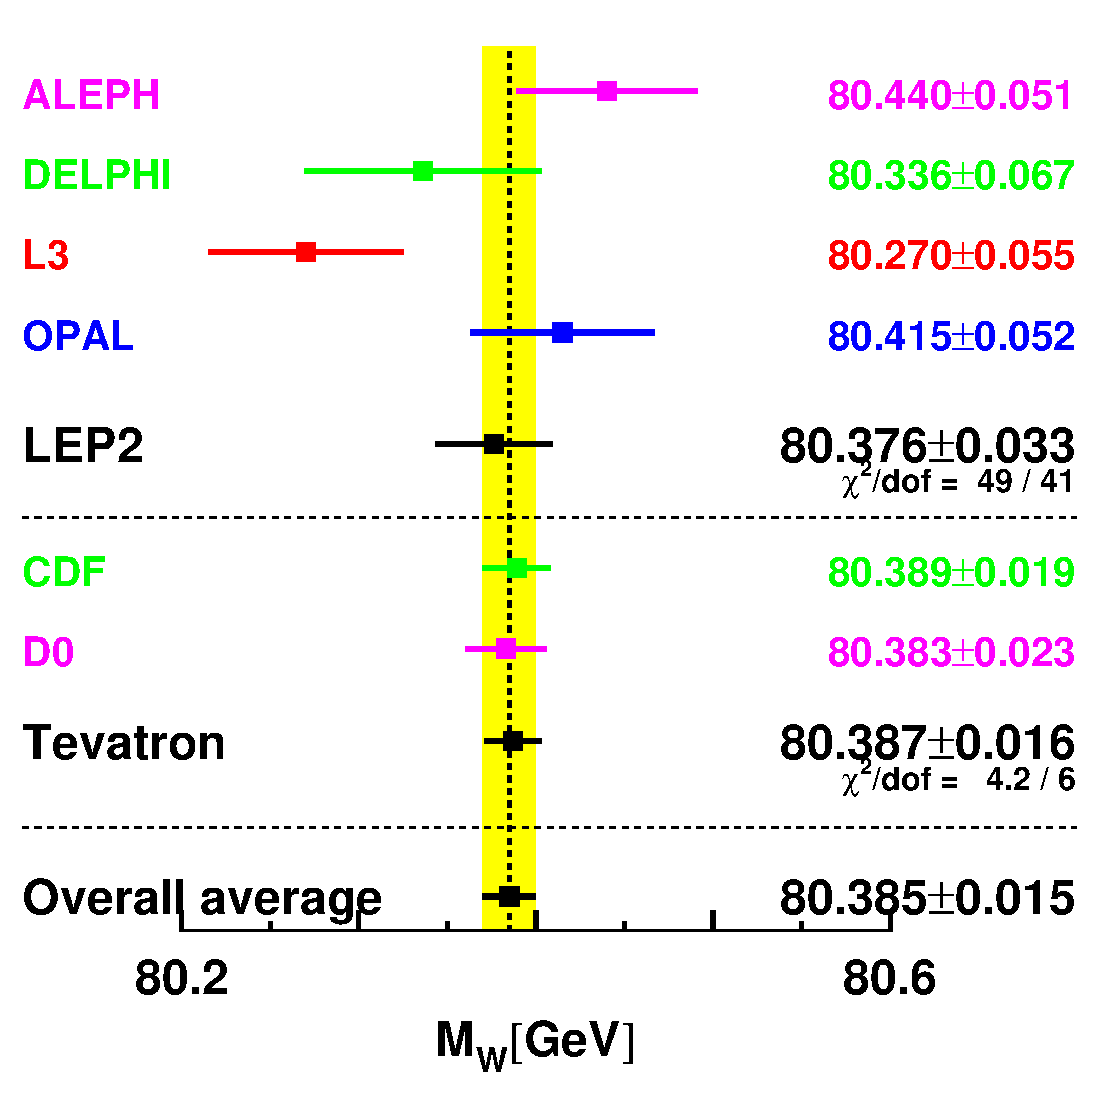
\includegraphics[width=.45\textwidth]{figures/theory/wmass_pdg.eps}
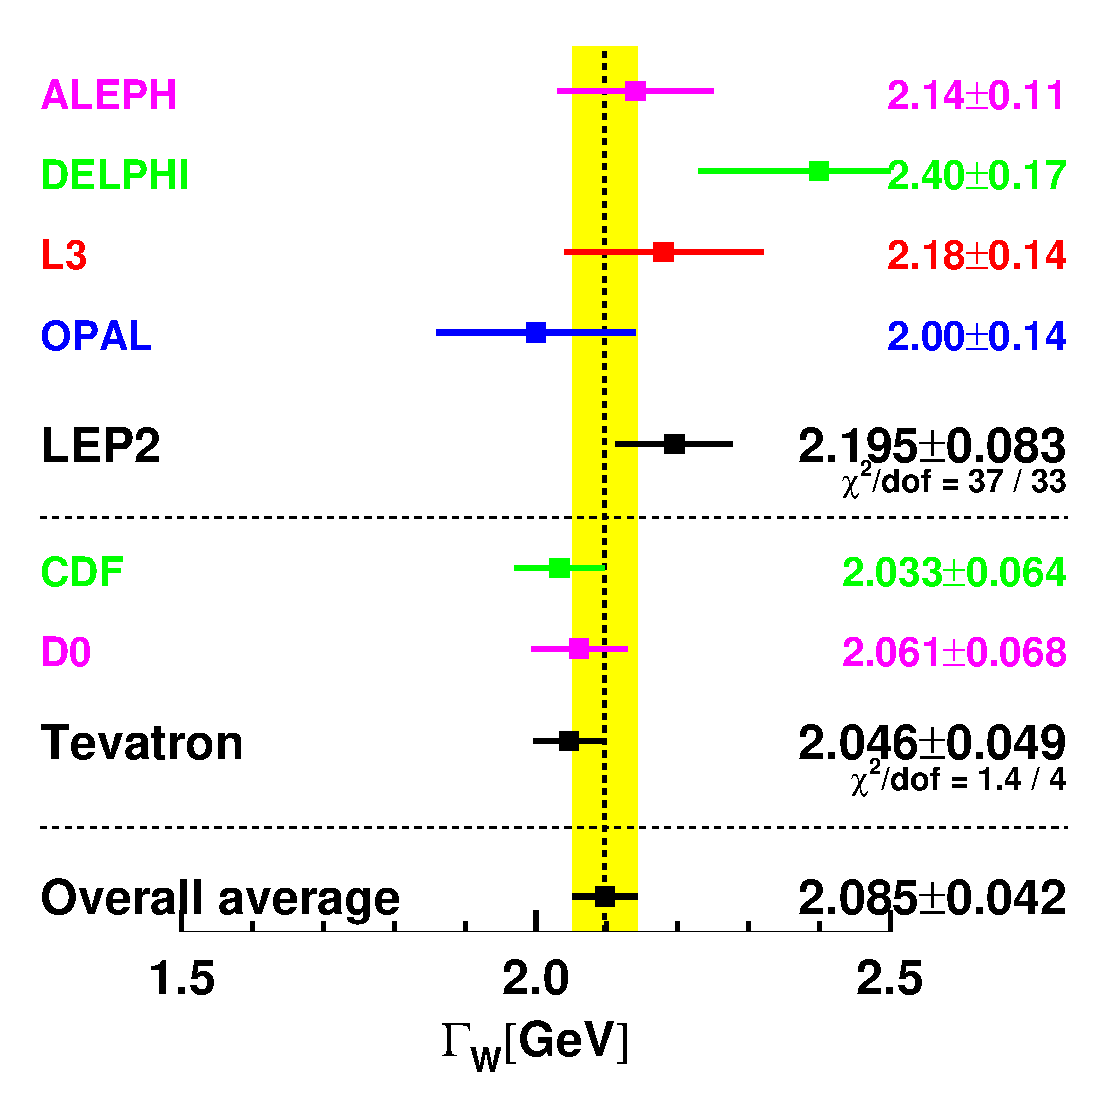
\includegraphics[width=.45\textwidth]{figures/theory/wwidth_pdg.eps}
\caption{Summary of \dubya~mass (left) and width (right) meassurements
as performed at LEP and the Tevatron~\cite{PDG:2014}.}
\label{fig:theory_w_pdg}
\end{figure}

Roughly 1/3 of of the time the \dubya~decays approximately 
evenly into each of the three lepton generations,
as expected from lepton universality.
The leptonic decays of the \dubya~result in a charged lepton 
with the same charge as the parent \dubya~(as dictated by charge conservation)
and a neutrino (or anti-neutrino if the parent \dubya~has negative charge).
Thus, the allowed leptonic decays are of the form:
\begin{align*}
W^{-} &\rightarrow l^{-} \overline{\nu}_l \\
W^{+} &\rightarrow l^{+} \nu_l
\end{align*}
The \dubya~decays into quarks the remaining 2/3 of the time with a positively
(negatively) chared \dubya~decaying into a up-type quark (anti-quark) and 
and down-type anti-quark (quark) as determined by charge conservation as follows:
\begin{align*}
W^{+} &\rightarrow q_u \overline{q}_d \\
W^{-} &\rightarrow \overline{q}_u q_d
\end{align*}
The \dubya~decay prefers decays into quarks/anti-quark pairs of the same generation.
However, quark universality is partially in the weak charged interactions, with
a slight mixing of the interactions between the three generations. The 
degree of mixing is described by the CKM matrix (cite) which has been
determined experimentally.  In general, this mixing of the three quark 
generations does not preserve CP symmetry. (define?) Indeed, small CP
violating effects were first observed in the weak interactions in 1964
by looking at the properties of kaon decays (cite, confirm wording).
The measured branching fractions for the \dubya~are 
summarized in \tab\ref{tab:theory_wdecay}.

maybe show feynman diagrams for W decay?

\begin{table}[ht]
\centering
\begin{tabular}{l|c}
Decay Mode &  Branching Fraction [\%]\\
\hline
$e^+\nu_e$ ($e^-\overline{\nu}_e$) & $10.71 \pm 0.16$ \\
$\mu^+\nu_{\mu}$ ($\mu^-\overline{\nu}_{\mu}$) & $10.63 \pm 0.15$\\
$\tau^+\nu_{\tau}$ ($\tau^-\overline{\nu}_{\tau}$) & $11.38 \pm 0.21$\\
Quarks & $67.41 \pm 0.27$\\
\end{tabular}
\caption{Measured branching fractions of the $\dubya^+$ ($\dubya^-$)~boson 
as reported by the Particle Data Group \cite{PDG:2014}.  The $W$ decays
to quarks result in hadronic states which in general prohibit
one from determining the specific $W$ final state. Thus, only 
an inclusive branching fraction is listed for the decay to quarks.}
\label{tab:theory_wdecay}
\end{table}


The cross-section of the production of the \dubya~at colliders
depends on the initial state (i.e. $pp$ vs $p\overline{p}$) and on the
collision energy. 
The cross-section times branching fraction to leptons 
has been measured thoroughly, with separate measurements performed
at RHIC~\cite{PhysRevLett.106.062001};
the SPS~\cite{Albajar1987271,Alitti1992365};
the Tevatron~\cite{0954-3899-34-12-001,D0-4403-CONF};
and most recently at the LHC 
at 7~\TeV~\cite{PhysRevD.85.072004,Chatrchyan:1370079}, 
8~\TeV~\cite{PhysRevLett.112.191802}, 
and 13~\TeV~\cite{ATLAS-CONF-2015-039,CMS-PAS-SMP-15-004}. 
A summary of these measurements is shown in 
\fig\ref{fig:theory_wxsec} which reveals them to be in good agreement with 
the predictions.

\begin{figure}[ht]
\centering
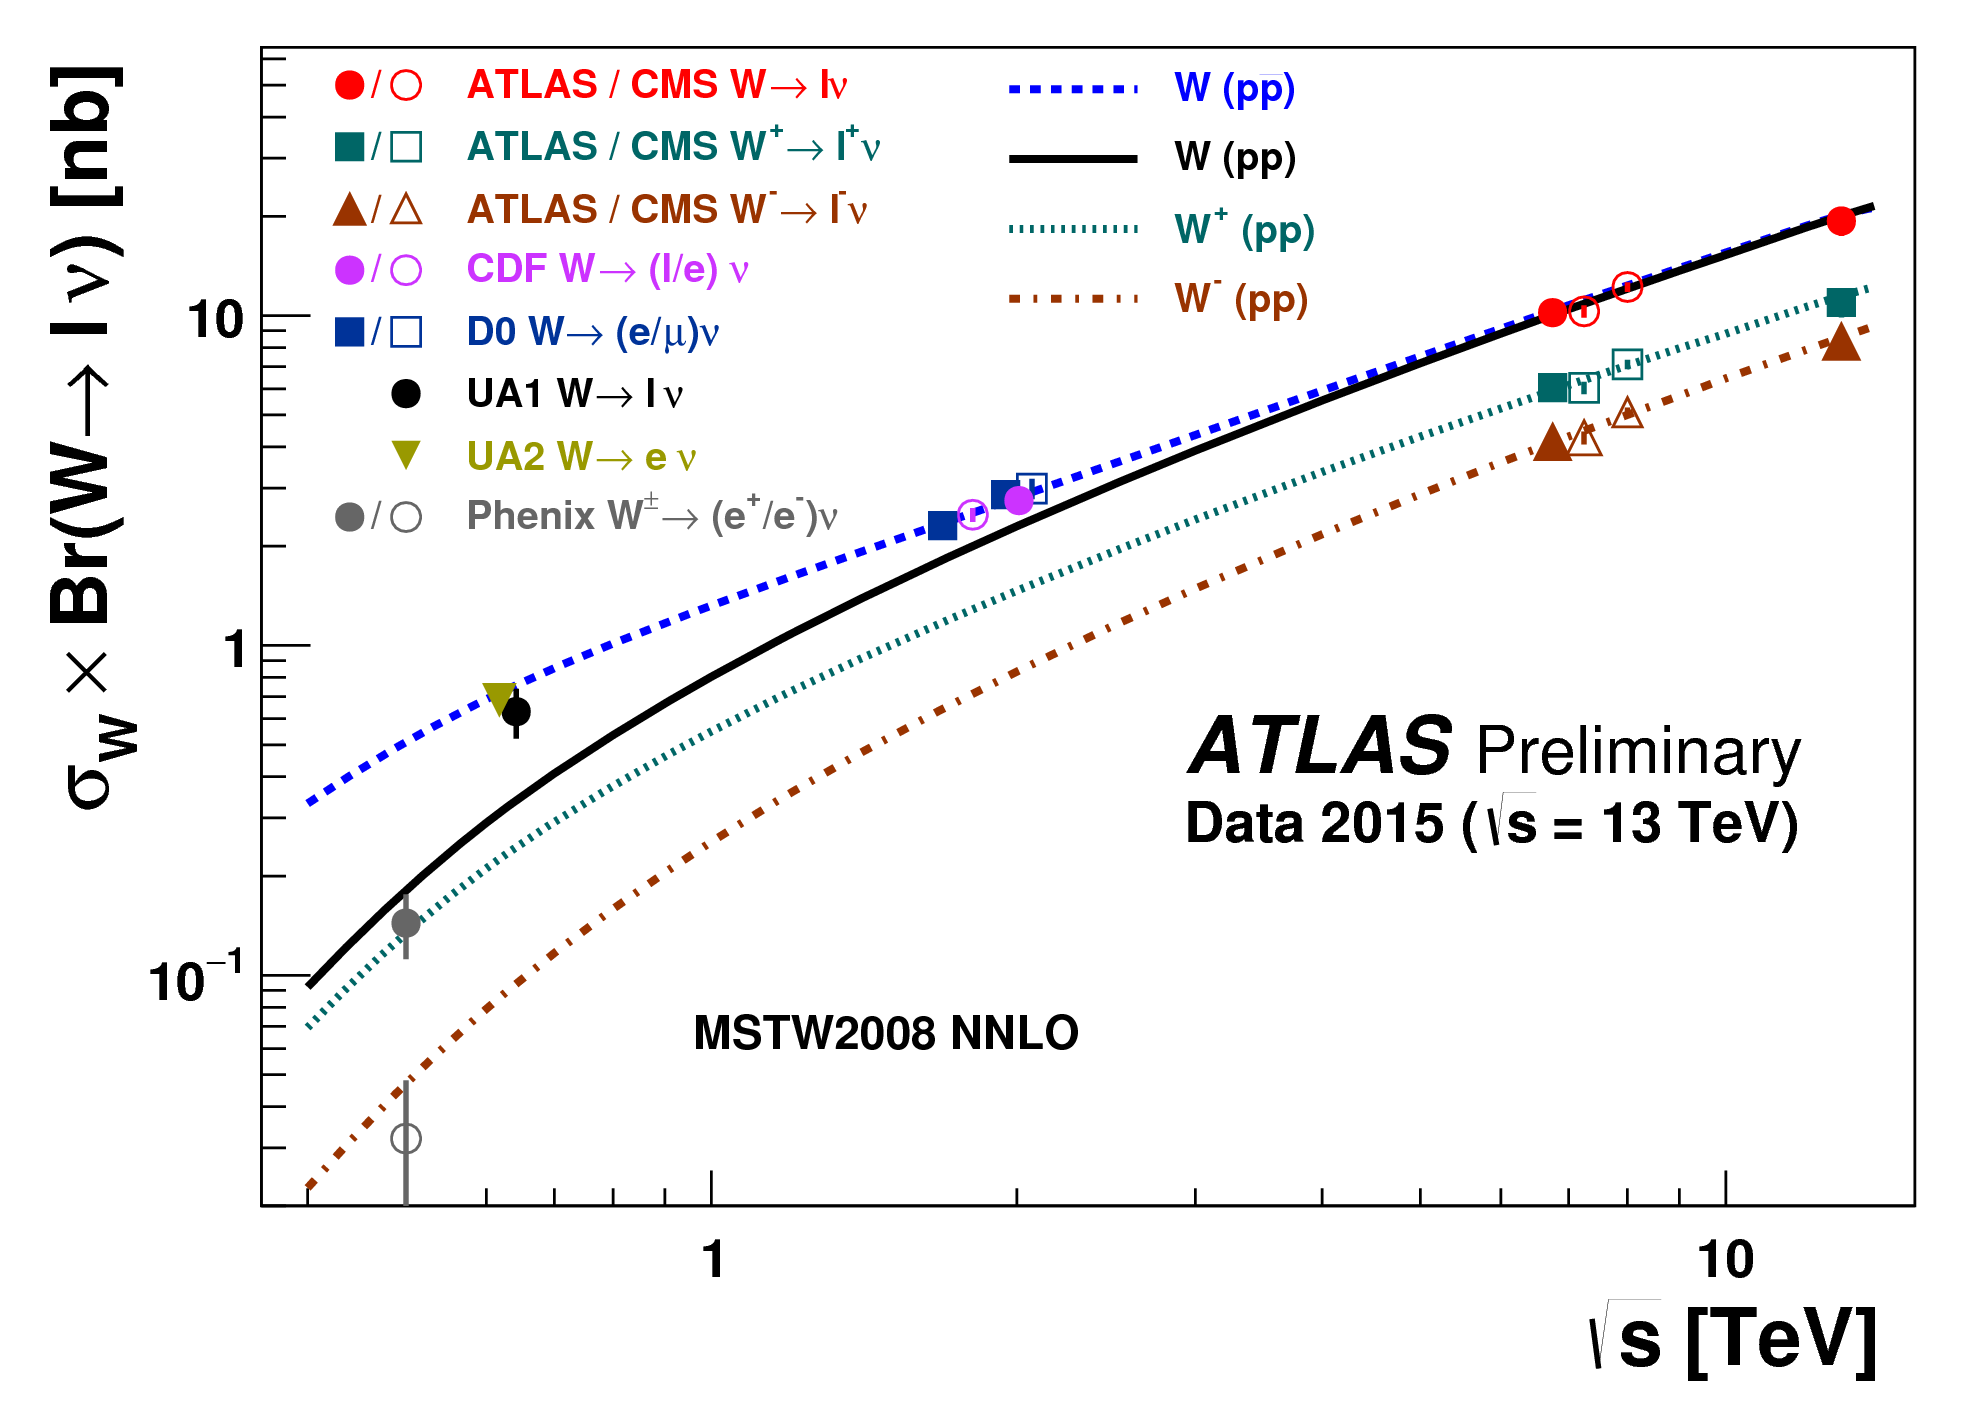
\includegraphics[width=.8\textwidth]{figures/theory/wxsec.png}
\caption{Summary of $W\rightarrow l\nu$ cross-section measurements as 
a function of center-of-mass energy, $\sqrt{s}$. 
Next-to-next-to-leading-order (NNLO) theoretical
predictions are shown for both $pp$ and 
$p\overline{p}$ collisions and for $pp$ collisions when split by charge.
Experimental measurements are overlayed and taken from measurements
at the SPS, RHIC, the Tevatron, and the LHC.  The plot is taken
from the ATLAS publication of $W$ and $Z$ cross-section measurements
at the LHC \cite{ATLAS-CONF-2015-039}.  }
\label{fig:theory_wxsec}
\end{figure}

Differential distributions?





\section{$WWW$ Production}

\unitlength = 0.6mm %necessary for feynmp
\begin{figure}[ht]
\centering
\vspace{5 mm}
\begin{fmffile}{feynwwwprod1}
		\begin{fmfgraph*}(80,50)
			\fmfleft{i1,i2}
			\fmfright{o1,o2,o3}

			\fmf{fermion}{i1,v1}
			\fmf{fermion}{v1,i2}
			\fmf{photon}{v1,v2}
			\fmf{photon}{v2,o1}
			\fmf{photon}{v2,o2}
			\fmf{photon}{v2,o3}
		\end{fmfgraph*}
\end{fmffile}
\hspace{6 mm}
\begin{fmffile}{feynwwwprod2}
		\begin{fmfgraph*}(80,50)
			\fmfleft{i1,i2}
			\fmfright{o1,o2,o3}

			\fmf{fermion}{i1,v1}
			\fmf{fermion}{v1,i2}
			\fmf{photon}{v1,v2}
			\fmf{photon}{v2,o1}
			\fmf{dashes,label=$H^0$}{v2,v3}
			\fmf{photon}{v3,o2}
			\fmf{photon}{v3,o3}
		\end{fmfgraph*}
\end{fmffile}

\vspace{6 mm}
\begin{fmffile}{feynwwwprod3}
		\begin{fmfgraph*}(80,50)
			\fmfleft{i1,i2}
			\fmfright{o1,o2,o3}

			\fmf{fermion}{i1,v1}
			\fmf{fermion}{v1,v2}
			\fmf{fermion}{v2,v3}
			\fmf{fermion}{v3,i2}
			\fmf{photon}{v1,o1}
			\fmf{photon}{v2,o2}
			\fmf{photon}{v3,o3}
		\end{fmfgraph*}
\end{fmffile}
\hspace{6 mm}
\begin{fmffile}{feynwwwprod4}
		\begin{fmfgraph*}(80,50)
			\fmfleft{i1,i2}
			\fmfright{o1,o2,o3}
			\fmf{fermion}{i1,v1}
			\fmf{fermion}{v1,v2}
			\fmf{fermion}{v2,i2}
			\fmf{photon,label=$Z/\gamma^{*}$}{v2,v3}
			\fmf{photon}{v1,o1}
			\fmf{photon}{v3,o2}
			\fmf{photon}{v3,o3}
		\end{fmfgraph*}
\end{fmffile}
\vspace{2 mm}
\caption{The tree level Feynman diagrams 
for $WWW$ production. The incoming fermion
lines in each diagram consist of an
up-type quark (anti-quark) and down-type anti-quark (quark). Unless
otherwise specified, the curvy lines correspond to $W$ bosons.}
\label{fig:theory_feynman_www}
\end{figure}

In this thesis, we are interested in the inclusive production of three
$W$ bosons from proton-proton collisions:
$pp\rightarrow\- \Wp\Wp\Wm+X$ and $pp\rightarrow \Wp\Wm\Wm\allowbreak +X$, 
where $X$ is intended to refer to the fact that no requirements are 
placed on additional particles produced in the hard interaction.
This is sensitive both
to the $WWWW$ coupling (non-resonant production) 
and to associated Higgs production \footnote{Associated Higgs production involves
the radiation of a Higgs boson off another particle (in this case a $W$ boson). It 
is sometimes referred to as ``Higgsstrahlung'', by analogy 
with electron Bremsstrahlung where an electron radiates a photon.} where 
the Higgs decays to two
$W$ bosons (resonant production). 
The relevant
tree-level feynman diagrams for this production process are shown in 
\fig\ref{fig:theory_feynman_www}.
The Higgs decay results in one $W$ boson being produced off-shell,
$H\rightarrow WW^*$, making this the leading contribution to off-shell
production.  
The resonance from the Higgs can clearly be seen from the 
distribution of $m_{\Wp\Wm}$ taken from the simulation of production \www~events
in \fig\ref{fig:mww_higgs}.

%It would be nice to show a plot of the Higgs stuff. maybe I can
%steal this and make my own later...
\begin{figure}[ht]
\centering
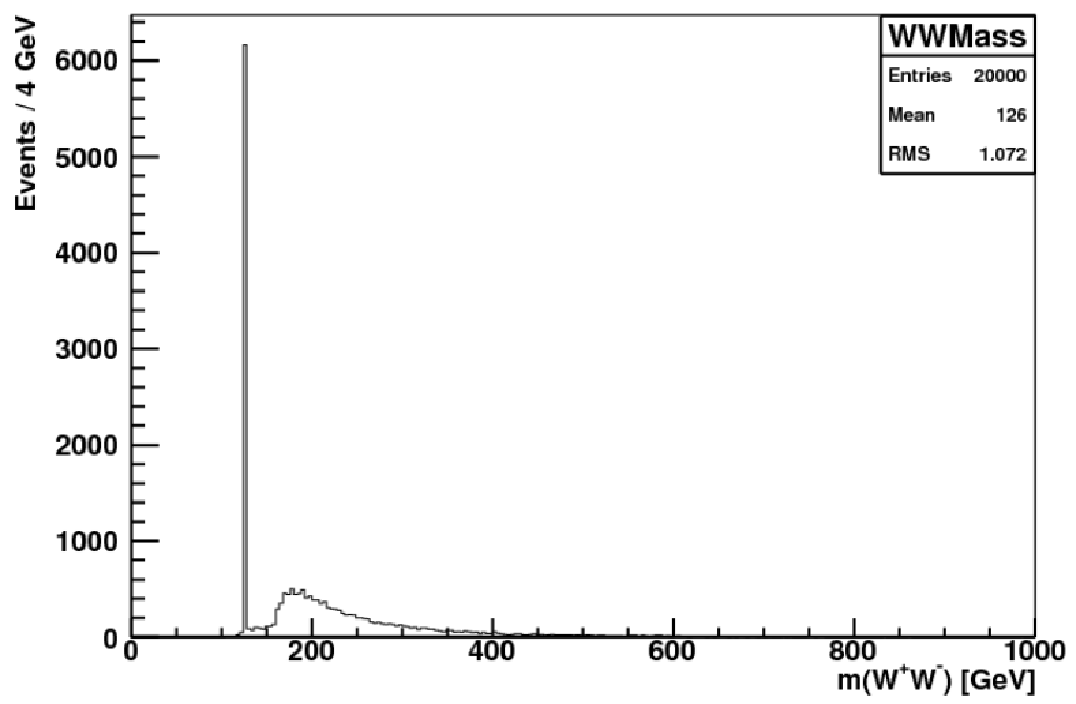
\includegraphics[width=0.5\columnwidth]{figures/2l2j/mWW-parton.pdf}
\caption{ Invariant mass distribution of two opposite-sign $W$ bosons 
in \www events generated with VBFNLO at LO. The Higgs mass peak is clearly 
visible at 126~GeV. (make a better plot)}
\label{fig:mww_higgs}
\end{figure}




The cross-section for this process can be computed at 
next-to-leading-order (NLO) in QCD
( $O(\alpha_s^2)$ in perturbation theory (?) ). 
(Mention more details of how this is computed like pdfs,
hadronization, interaction, radiation, decays. Use one of the 
feynman diagrams)
Using 
the \madgraph~generator finds an inclusive cross-section of 
\begin{equation}
\sigma(pp\rightarrow WWW + X) = 241.47 \pm 0.13~\textrm{fb}
\end{equation}
where the uncertainty is purely statistical.
The contribution from resonant production is computed separately
and found to make up about 64\% of the 
total inclusive cross-section.
More details on the determination of the signal cross-section, uncertainties,
and kinematics are presented in \sec\ref{sec:signal}.

\begin{figure}
\centering
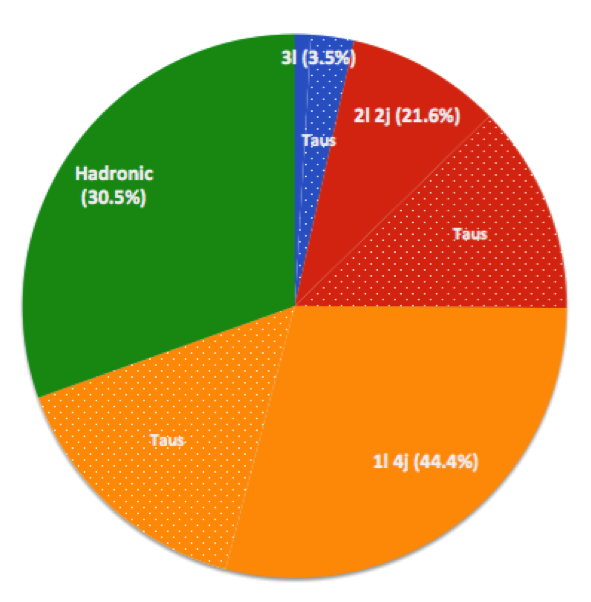
\includegraphics[scale=.8]{figures/branching_fractions.png}
\caption{Pie chart showing the different decay modes contributing 
to the total \xsec for the \www~process. 
The dotted areas indicate the portion of each decay 
mode which is due to the production of tau leptons.}
\label{fig:branching_fractions}
\end{figure}

Due to the short lifetime of the $W$ boson, each of the $W$ bosons
in the $WWW$ process will decay before reaching the detector.
This results in a measurable final state for the $WWW$ production 
process that includes some combination of leptons 
and quarks (manifested as jets).  The branching fractions for 
the $WWW$ process can be determined from the individual $W$ branching fractions
listed in \tab\ref{tab:theory_wdecay}.  The expected $WWW$ branching
fractions are thus summarized in the pie chart in \fig\ref{fig:branching_fractions}.
For this thesis, we are primarily interested in the final state
where each $W$ boson decays leptonically (the fully-leptonic final state) 
which has the smallest branching fraction at roughly 3.5\%.
In fact, since the $\tau$ leptons are also unstable, we choose to 
omit $W$ decays to $\tau$ leptons from our fully-leptonic
definition as well. This further reduces the fully-leptonic 
branching fraction to 0.97\%.  While small, this fully-leptonic final state
should have smaller backgrounds to the signal than the other 
decay channels, making it one of the most sensitive channels for studying
this process. The branching fraction when one $W$ boson is allowed
to decay hadronically is considerably larger, at 21.6\% (or
9.2\% when excluding decays to $\tau$ leptons). This is 
referred to as the semi-leptonic decay channel. The presence
of the two leptons from the other two $W$ decays still allows
for background discrimination, though not as much as in the fully-leptonic
channel. As a result, this channel has also been studied, though it 
is not the focus of this thesis. The remaining channels have
not been studied. The combination of the fully-leptonic
and semi-leptonic channels is presented in \sec\ref{sec:measurement}.



\section{Effective Field Theory}
\subsection{Anomalous Quartic Gauge Couplings}
%be sure to add a review of measurements

A measurement
of the production rate can be used to probe the gauge couplings, in
particular, the process is sensitive to quartic gauge couplings. The
{\sc VBFNLO } code has implemented a list of higher order operators
that parameterize the effects of new physics at energy scale beyond
the reach of current collider experiments.  The effective field theory
approach is practical and widely used when there is no compelling
specific model of new physics beyond the SM, see for example,
discussions in Refs:~\cite{Hagiwara:1993ck}, \cite{Buchmuller:1985jz}
and \cite{Eboli:2006wa}.  As a benchmark, we choose two gauge
invariant dimension-8 operators:
\begin{equation}
\mathcal{L}_{s,0} = [(\mathrm{D}_\mu\phi)^\dag\mathrm{D}_\nu \phi]\times [(\mathrm{D}^\mu\phi)^\dag\mathrm{D}^\nu \phi]
\end{equation}
\begin{equation}
\mathcal{L}_{s,1} = [(\mathrm{D}_\mu\phi)^\dag\mathrm{D}^\mu \phi]\times [(\mathrm{D}_\nu\phi)^\dag\mathrm{D}^\nu \phi]
\end{equation}
where $\phi$ is the Higgs field doublet, and $\mathrm{D}_\mu$ is the covariant derivative. 
The Lagrangian of the effective field theory is thus: 
\begin{equation}
\mathcal{L}_{eff} = \mathcal{L}_{SM} + \frac{f_{s0}}{\Lambda^4}\mathcal{L}_{s,0}+\frac{f_{s1}}{\Lambda^4}\mathcal{L}_{s,1}
\end{equation}
The choice of the two operators is introduced to benchmark possible
deviations from the SM. If a significant excess of events is 
observed in the data, the parameterization will be changed, to incorporate 
more operators, to
investigate the nature of the observed new physics.
% Once statistically significant
% deviation is observed, of course, more operators should be considered
% for investigating the nature of the observed new physics.


\section{Status of QGC Measurements and aQGC Limits}
A variety of measurements sensitive QGC interactions have been
performed at colliders. In particular, measurements sensitive
to $WW\gamma\gamma$ have been performed 
at LEP \cite{Abdallah:2003xn,PhysRevD.70.032005}, 
the Tevatron \cite{PhysRevD.88.012005}, %is this really the only tevatron measurement??
and the LHC \cite{PhysRevLett.115.031802,PhysRevD.90.032008,Chatrchyan:2013akv}; 
%mention how they were probed?
to $WWZ\gamma$ at LEP~\cite{Achard:2001eg,Abbiendi:1999aa,Abbiendi:2003jh}
and at the LHC~\cite{PhysRevD.90.032008};
to $ZZ\gamma\gamma$ at LEP \cite{Achard:2002iz,PhysRevD.70.032005}; 
and to $WWWW$ at the LHC \cite{PhysRevLett.113.141803,PhysRevLett.114.051801}. 
Typically, these studies are performed
by looking at x final state (more detail). 
The first measurements sensitive to the $WWWW$ vertex focused on 
same-sign $WW$ vector boson scattering because...

material on limits?

summary plots? maybe from pdg?


